In the following section we will showcase the resulting flow of our prototype and the evaluation results for our repository containing the QuixBugs benchmark problems.
\section{Showcase of workflow}

% To integrate the APR system into a repository living on GitHub we need to move the pipeline with its filter script to the dedicated github action workflow directory.
% ---IMAGE OF WORKFLOW IN PLACE
% % \begin{figure}[H]
% %     \centering
% %     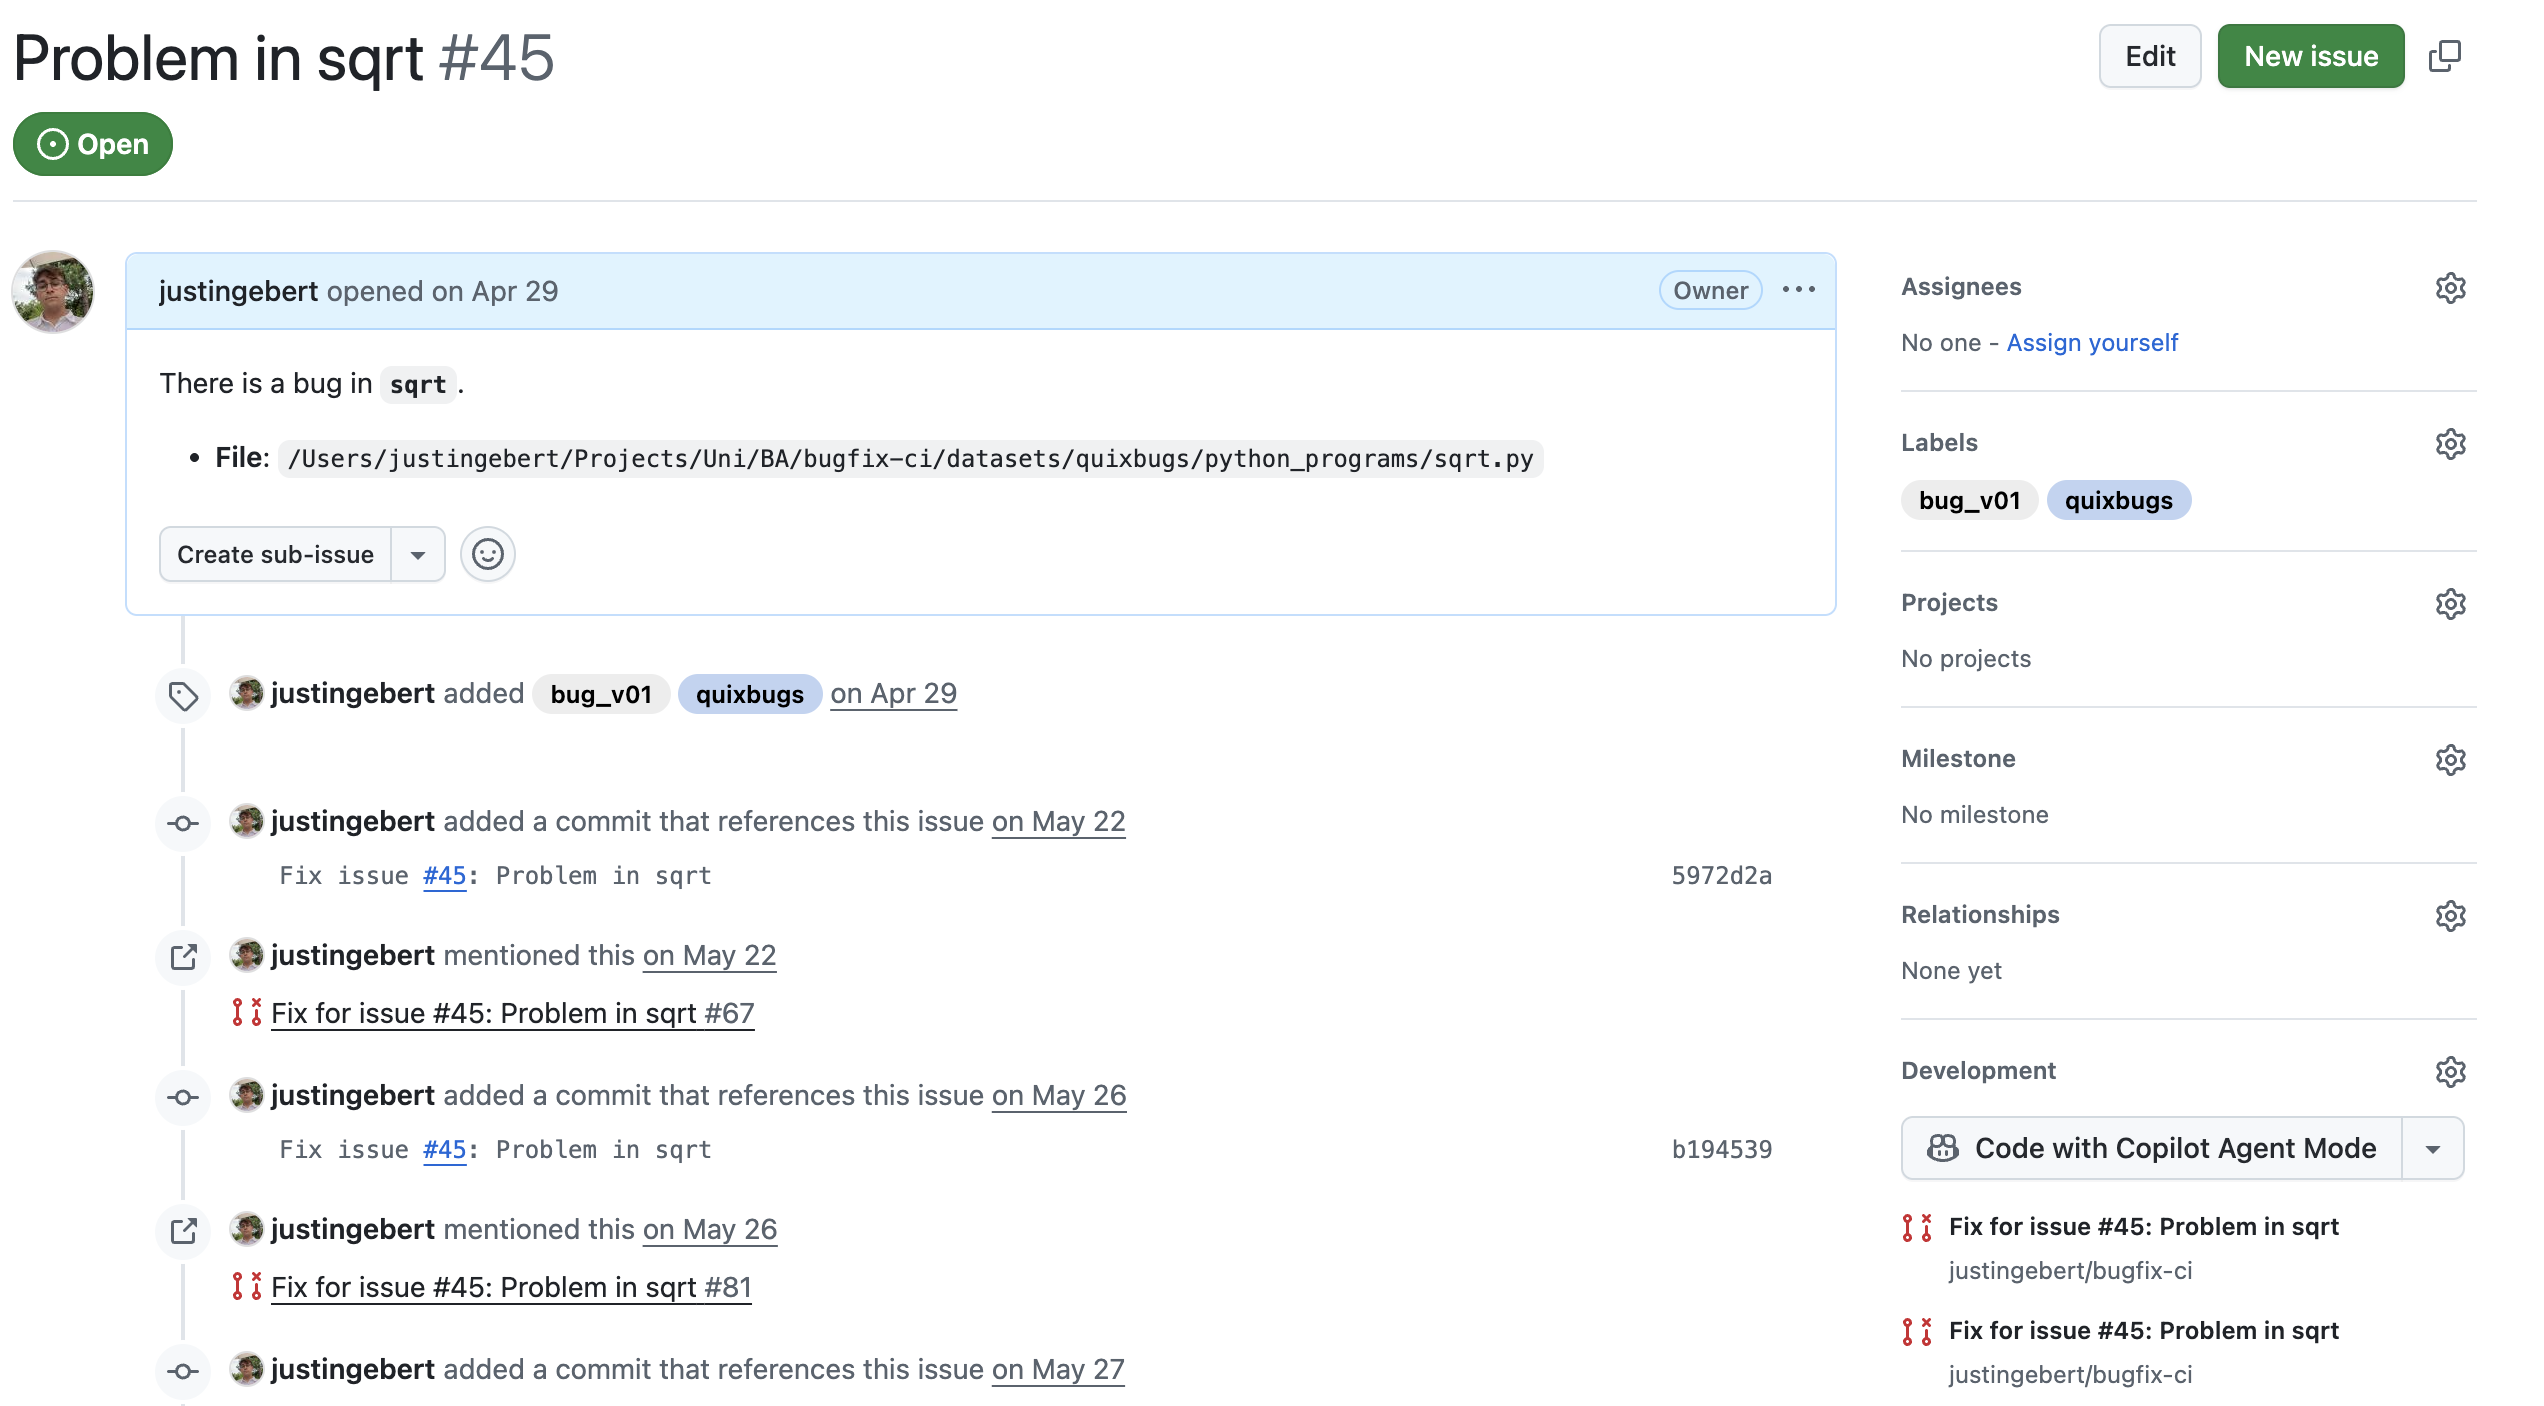
\includegraphics[width=1\textwidth]{images/github/GitHub Issue.png}
% %     \caption{Example of a GitHub Issue}
% %     \label{fig:gh-issue}
% % \end{figure}

% The follwing repository secrets need to be set in the repository settings GITHUB\_TOKEN: a personal access token with write access to the repository LLM\_API\_KEY: the API key for the LLM provider e.g. OpenAI, Gemini, etc.

% When the workflow is in place the APR system is ready to go. Optionally its default behavior can be altered by adding a configuration file (called: bugfix.yml) to the root of the repository.
% ---EXAMPLE OF CONFIG
% % \begin{figure}[H]
% %     \centering
% %     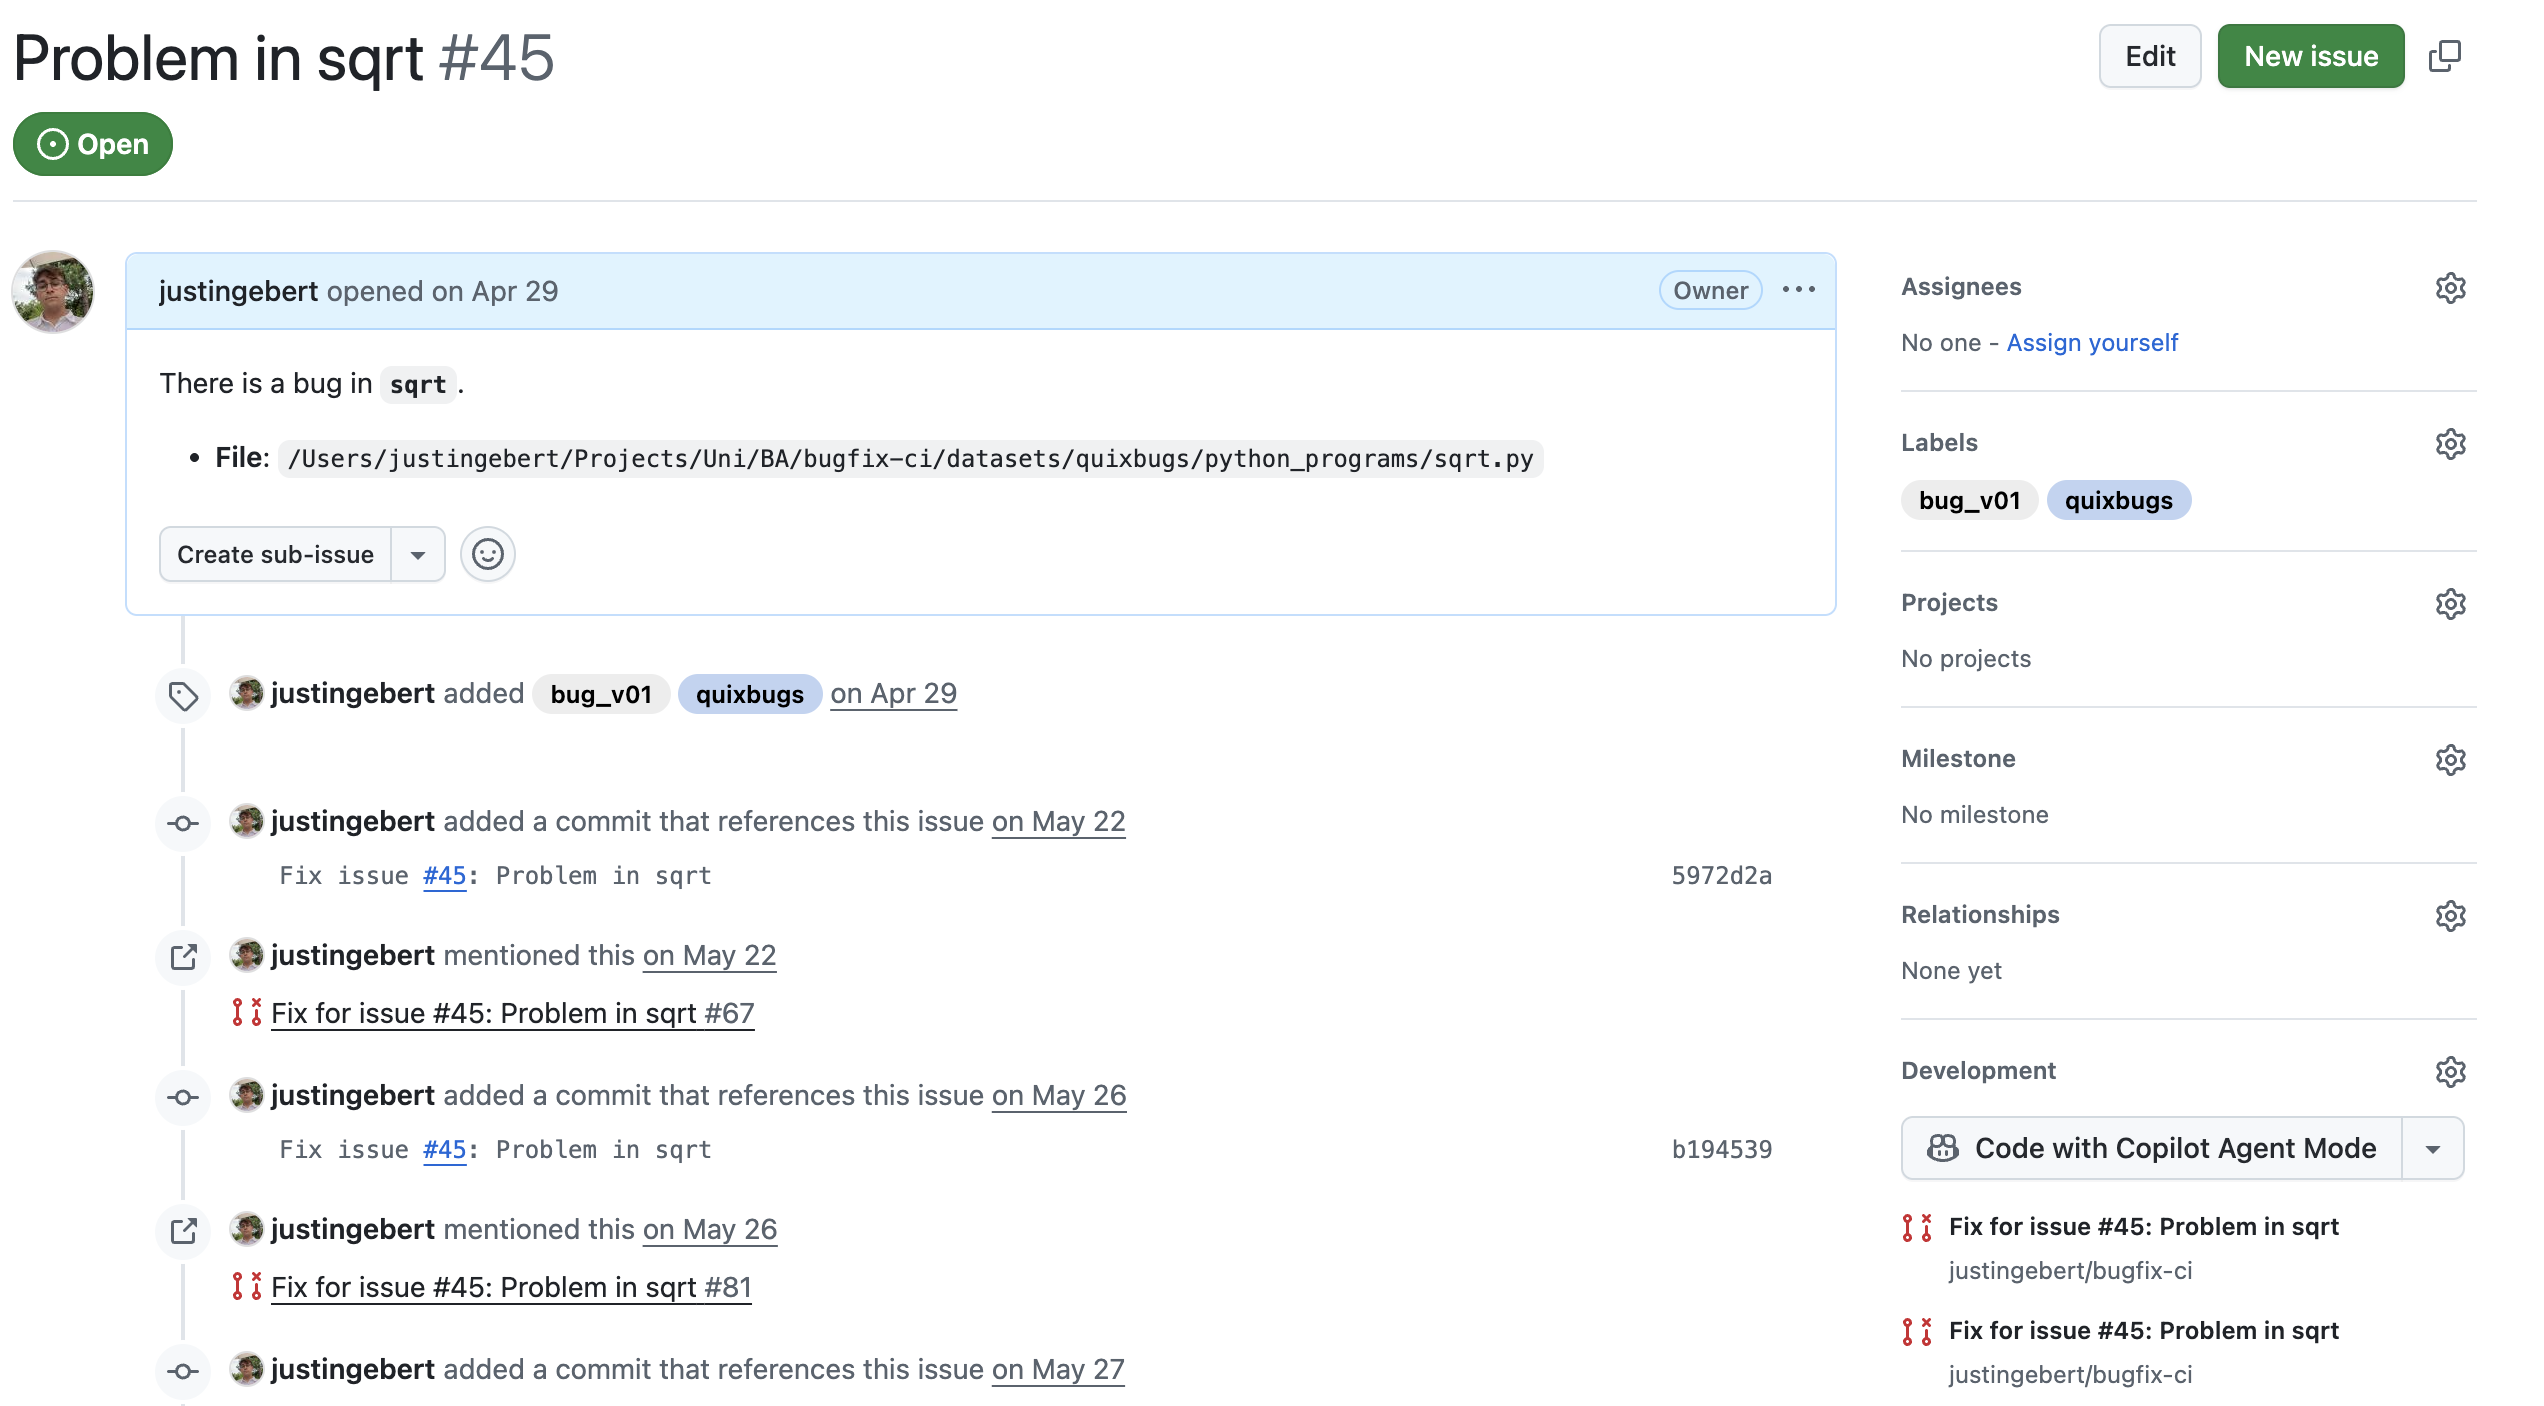
\includegraphics[width=1\textwidth]{images/github/GitHub Issue.png}
% %     \caption{Example of a GitHub Issue}
% %     \label{fig:gh-issue}
% % \end{figure}

With the system in place and the configuration file set up, the APR system is ready to be used in a repository.

\begin{figure}[H]
    \centering
    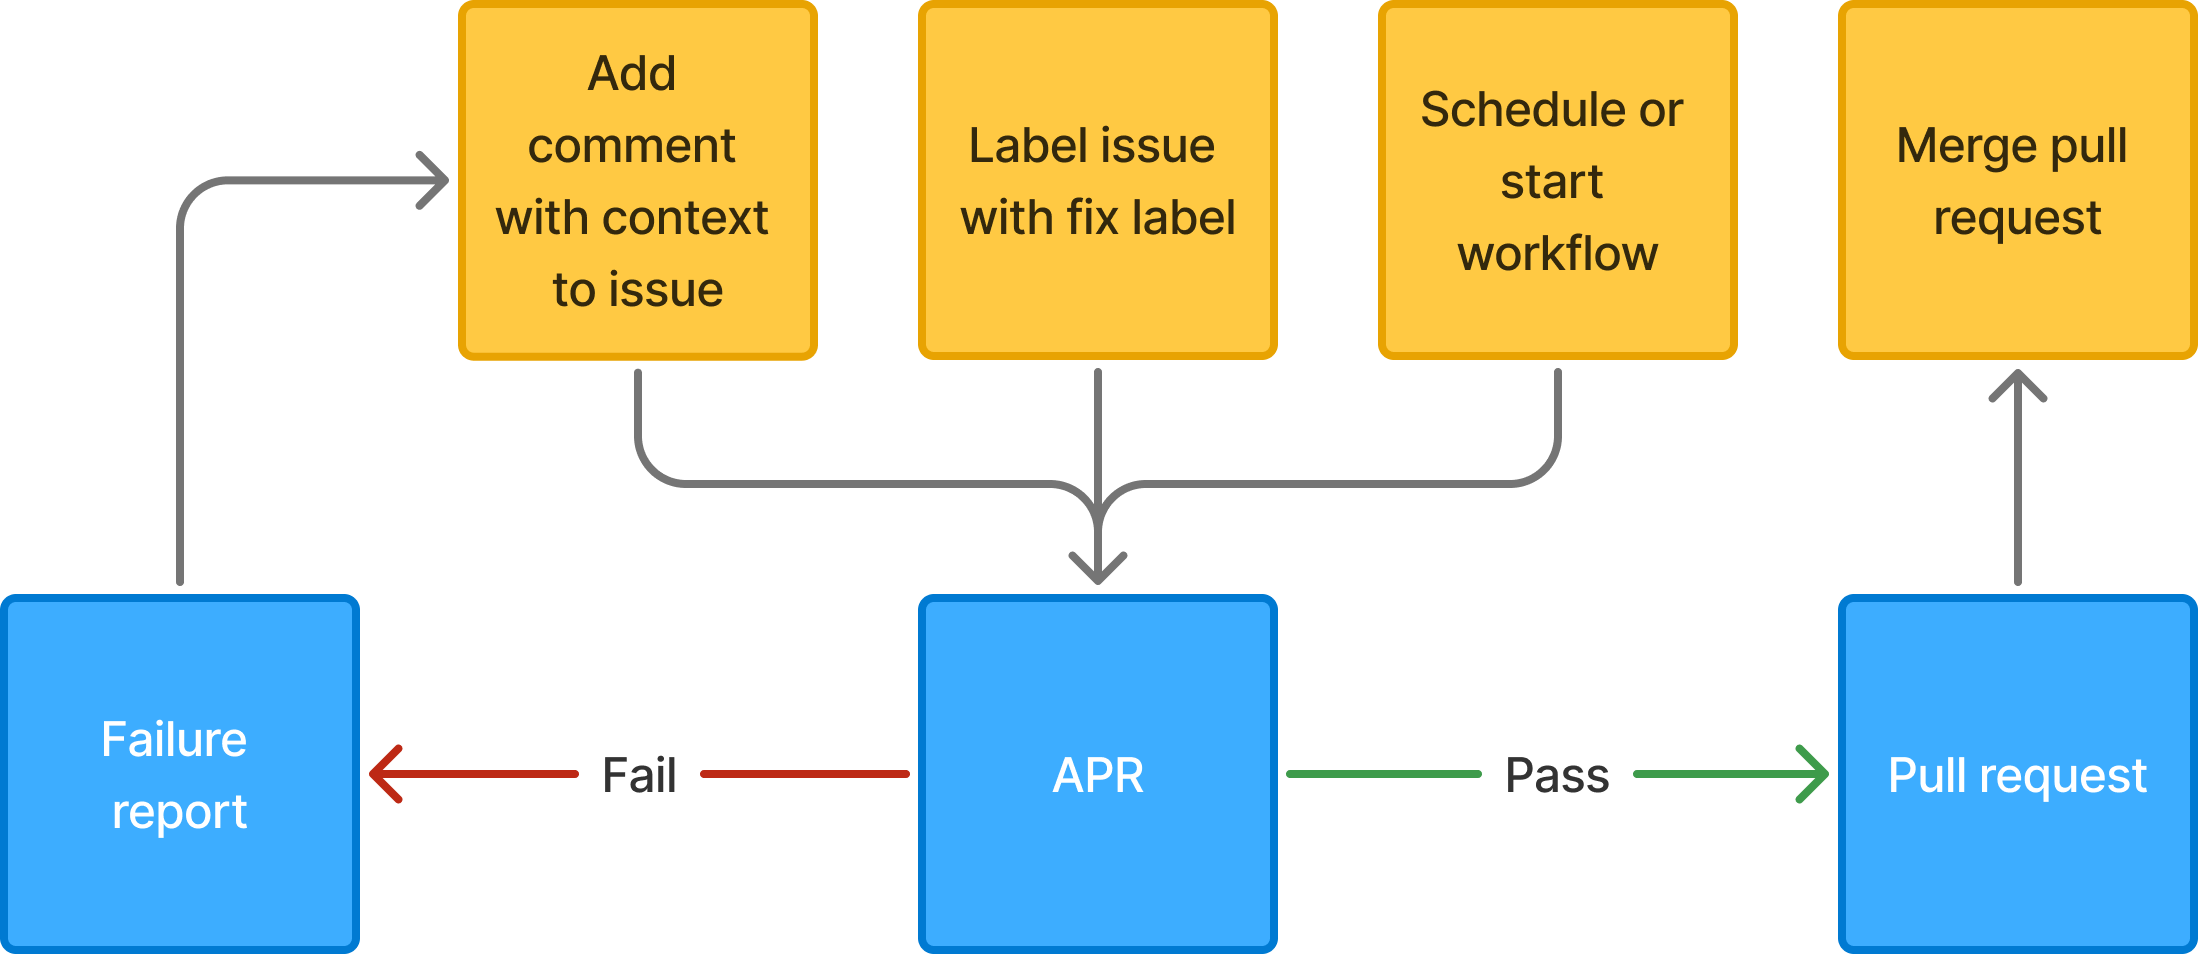
\includegraphics[width=0.9\textwidth]{images/flowcharts/flowresult.png}
    \caption{Resulting flow diagram}
    \label{fig:flow}
\end{figure}

Now when an issue is created and labeled with the default label "bug" (or a custom label defined in the configuration file) the APR system will be triggered and start the bug fixing process. Manual triggering is also possible by using the "Run workflow" button in the GitHub actions tab of the repository.
\begin{figure}[H]
    \centering
    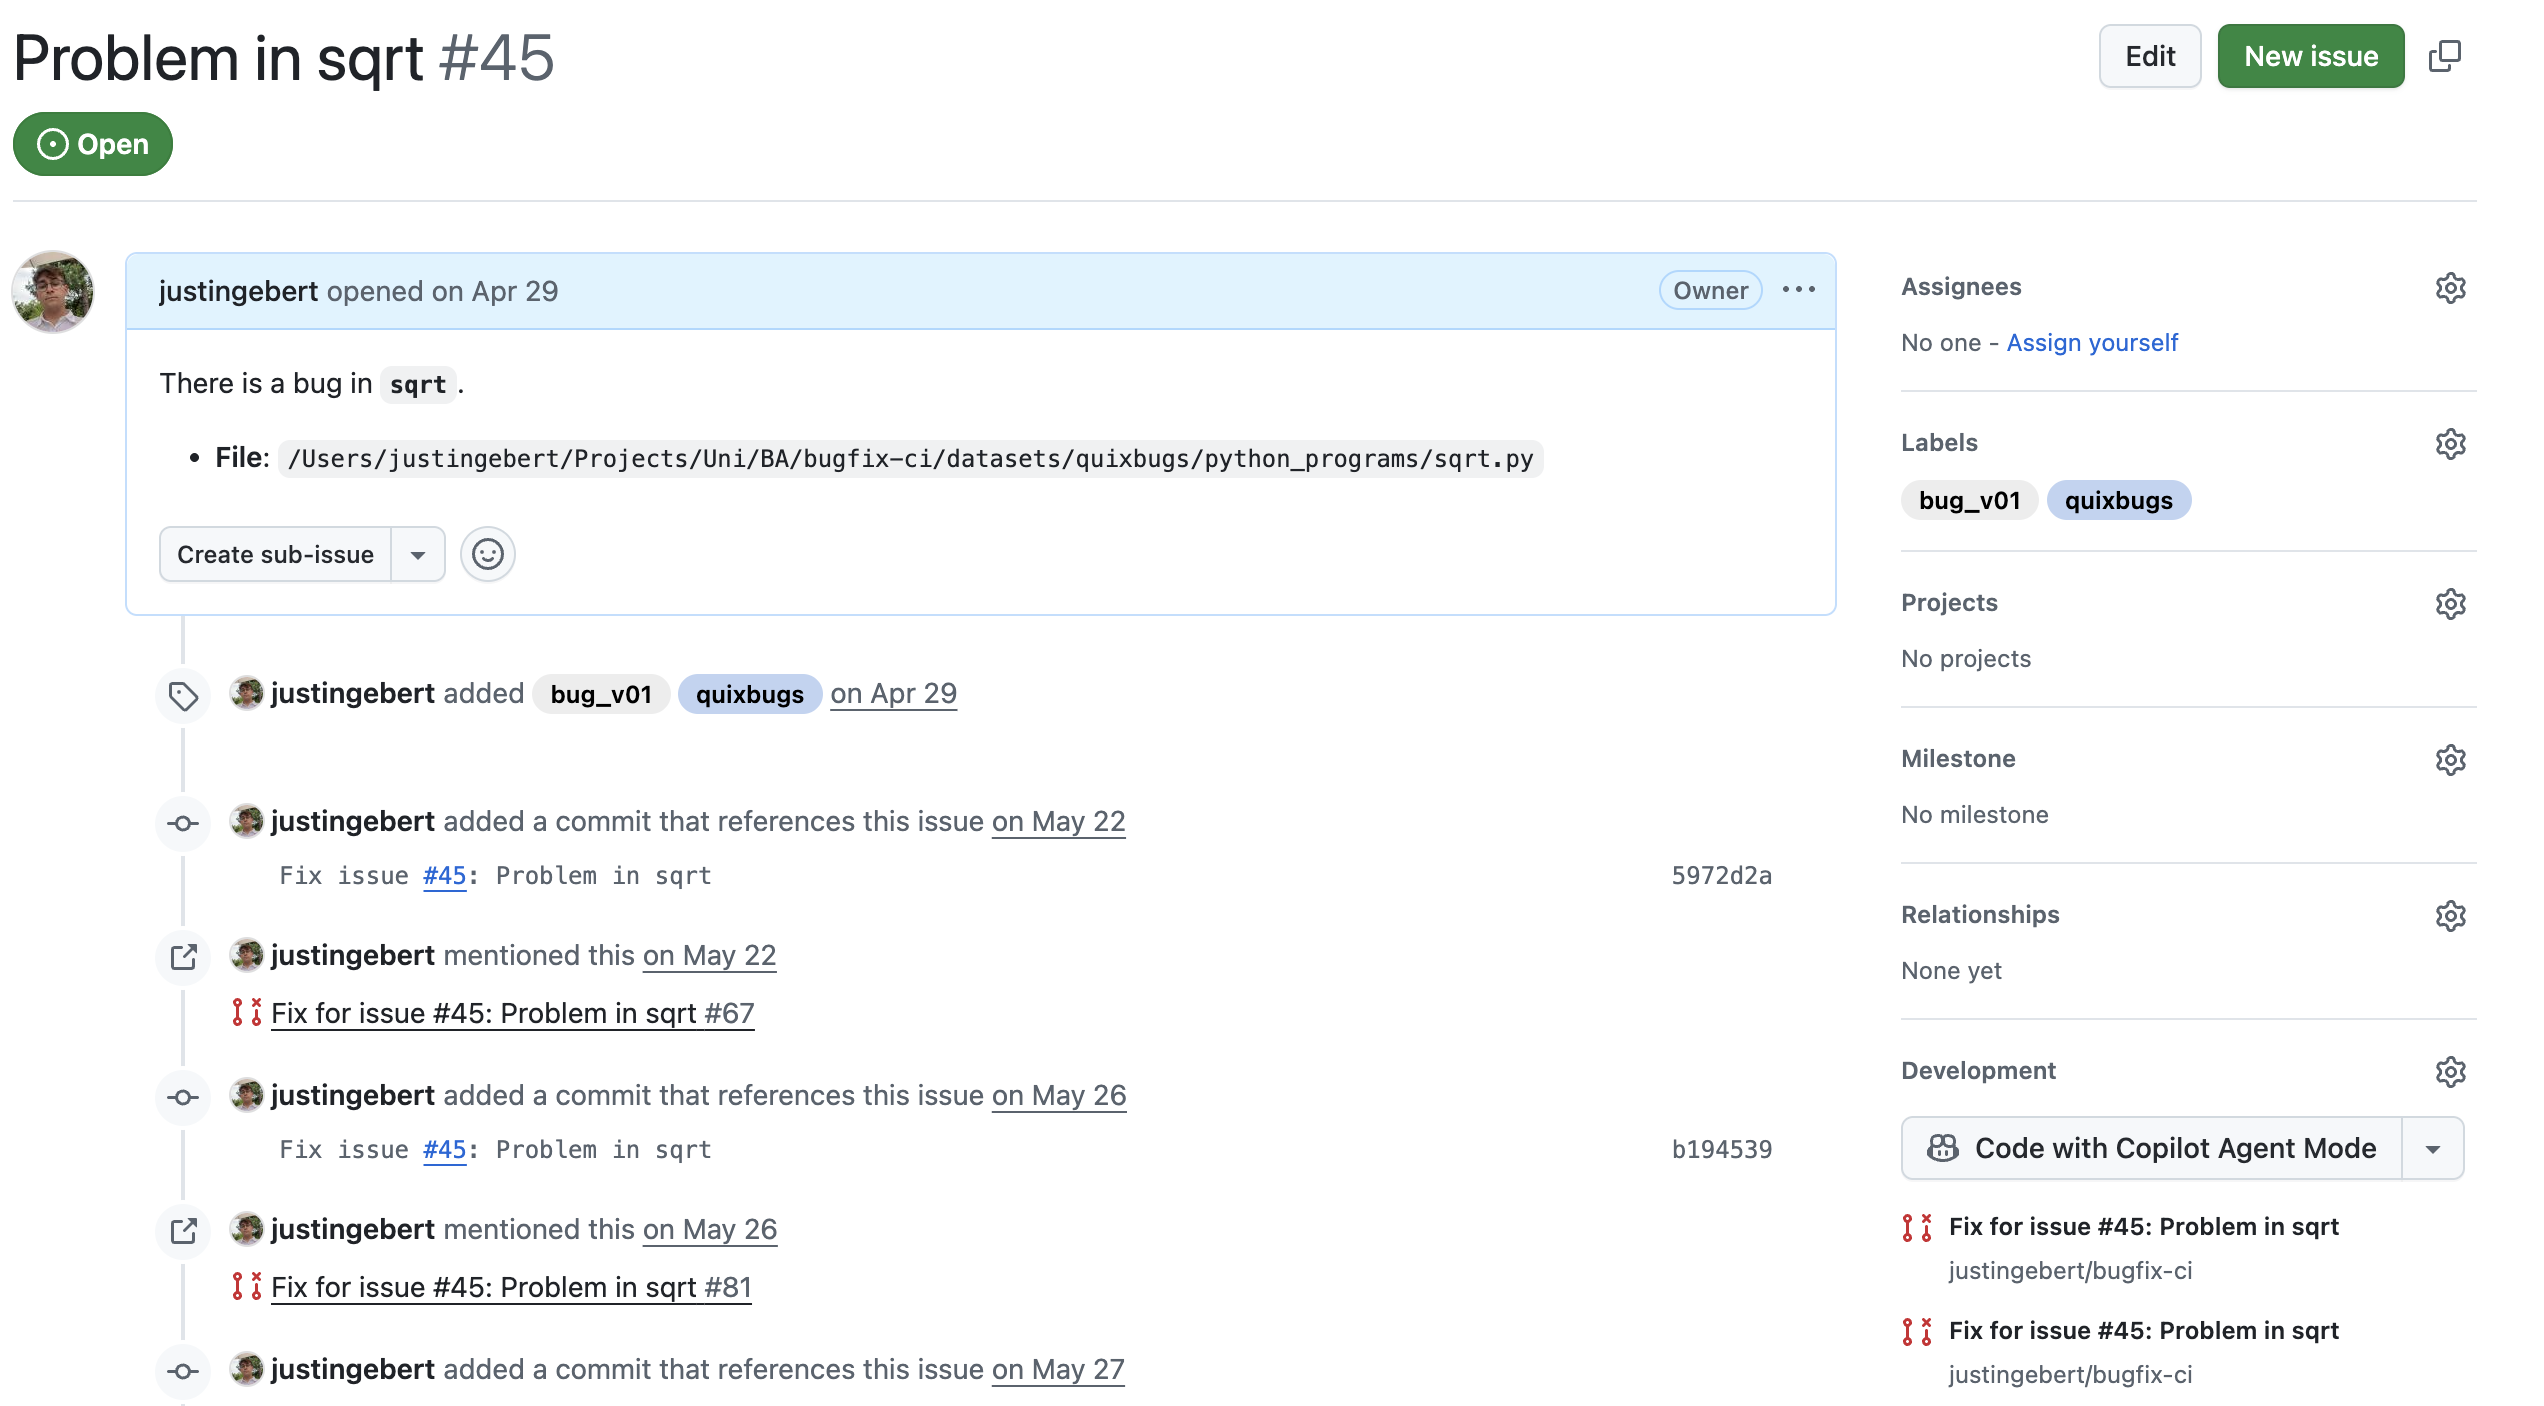
\includegraphics[width=1\textwidth]{images/github/GitHub Issue.png}
    \caption{GitHub Issue for APR}
    \label{fig:gh-issue-APR}
\end{figure}

After the workflow is triggered and relevant issues are found the APR system start as a run of the GitHub action workflow.
\begin{figure}[H]
    \centering
    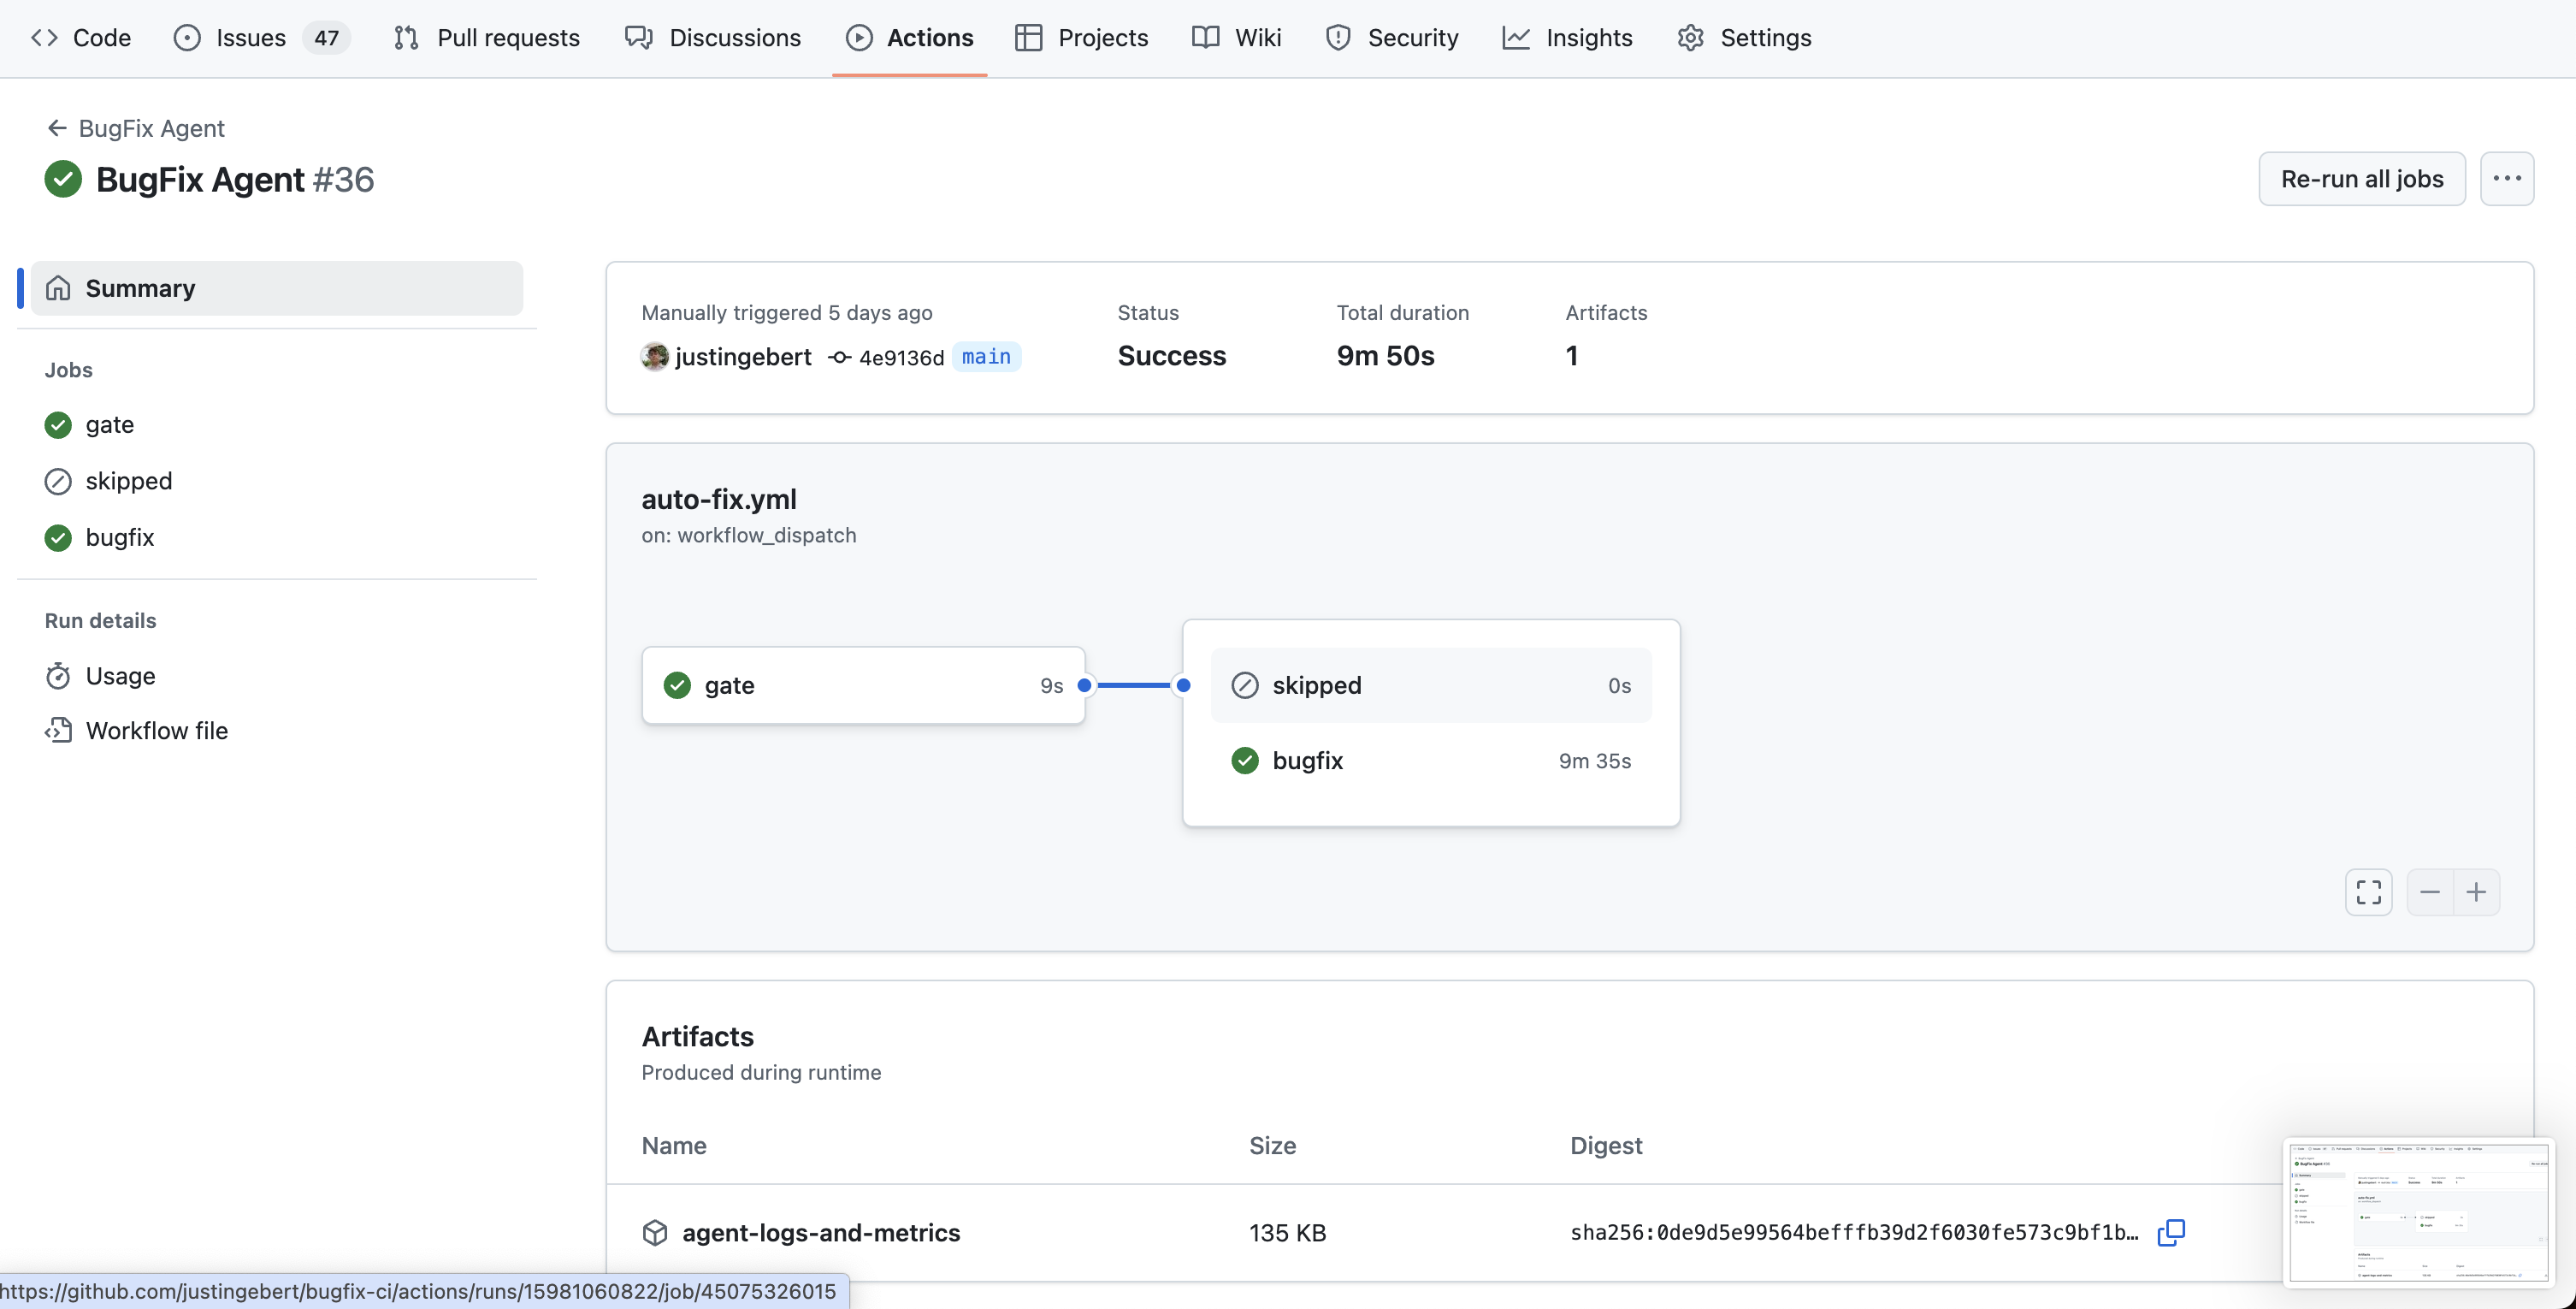
\includegraphics[width=1\textwidth]{images/workflow/Action.png}
    \caption{Example of a GitHub Issue}
    \label{fig:apr-action}
\end{figure}

When the bugfix step is executed Pull Requests will show up for the successfully fixed issues. A pull request shows the changes made to the codebase and the issue it is related to. The pull request can then be reviewed and merged.
\begin{figure}[H]
    \centering
    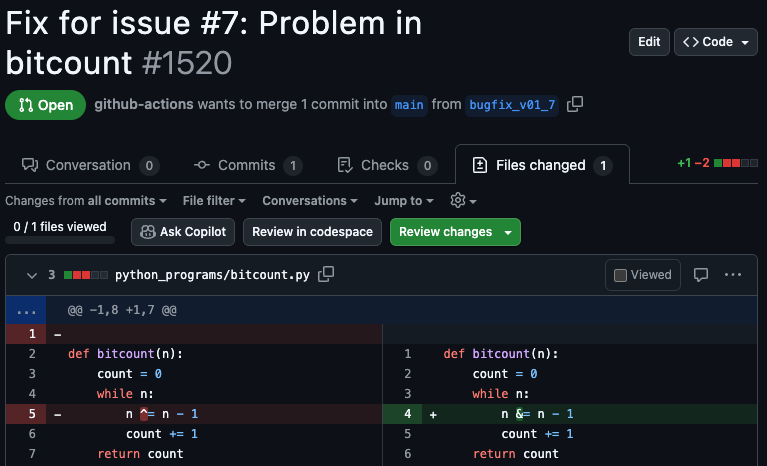
\includegraphics[width=1\textwidth]{images/workflow/PR.png}
    \caption{Resulting Pull Request}
    \label{fig:pr}
\end{figure}

If APR fails to fix an issue, it will report the failure in the GitHub issue as a comment and label it as fix failed.
\begin{figure}[H]
    \centering
    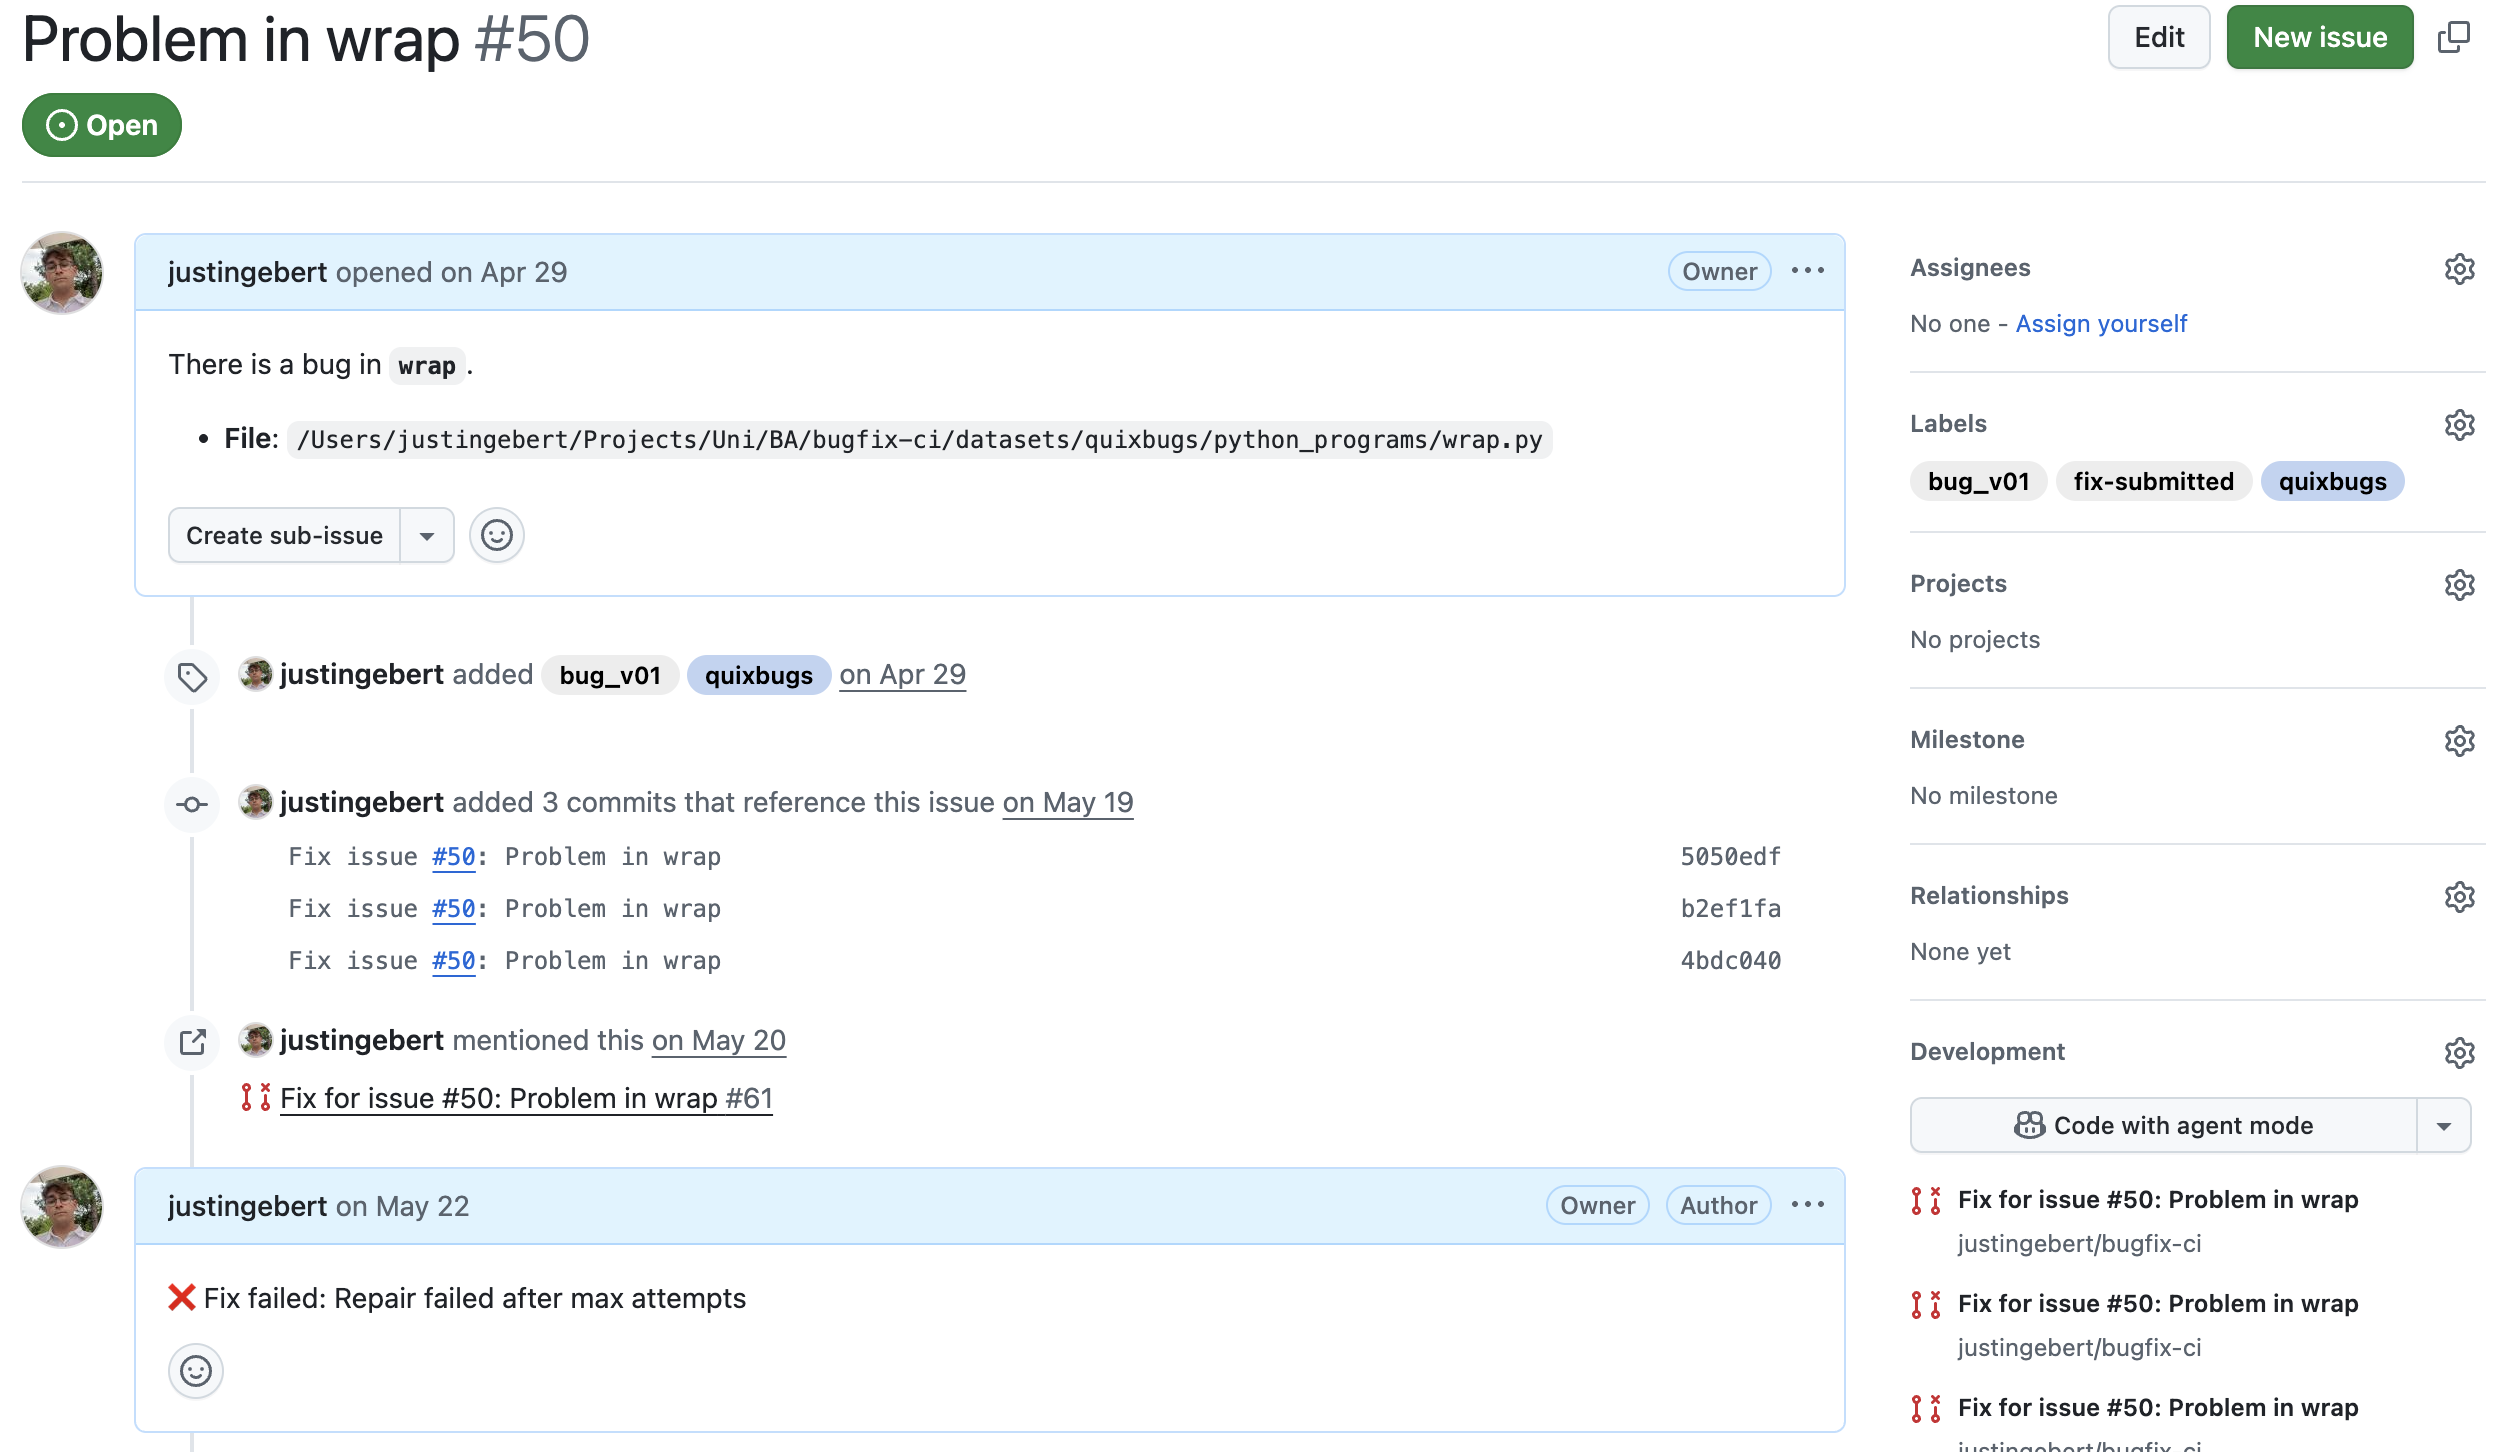
\includegraphics[width=1\textwidth]{images/workflow/issue comment.png}
    \caption{Failure Report}
    \label{fig:failure-report}
\end{figure}

During a run logs are live streamed in the Workflow run seen in \ref{fig:log-stream}.  When completed, logs and metrics are available for download in the action as artifacts.
\begin{figure}[H]
    \centering
    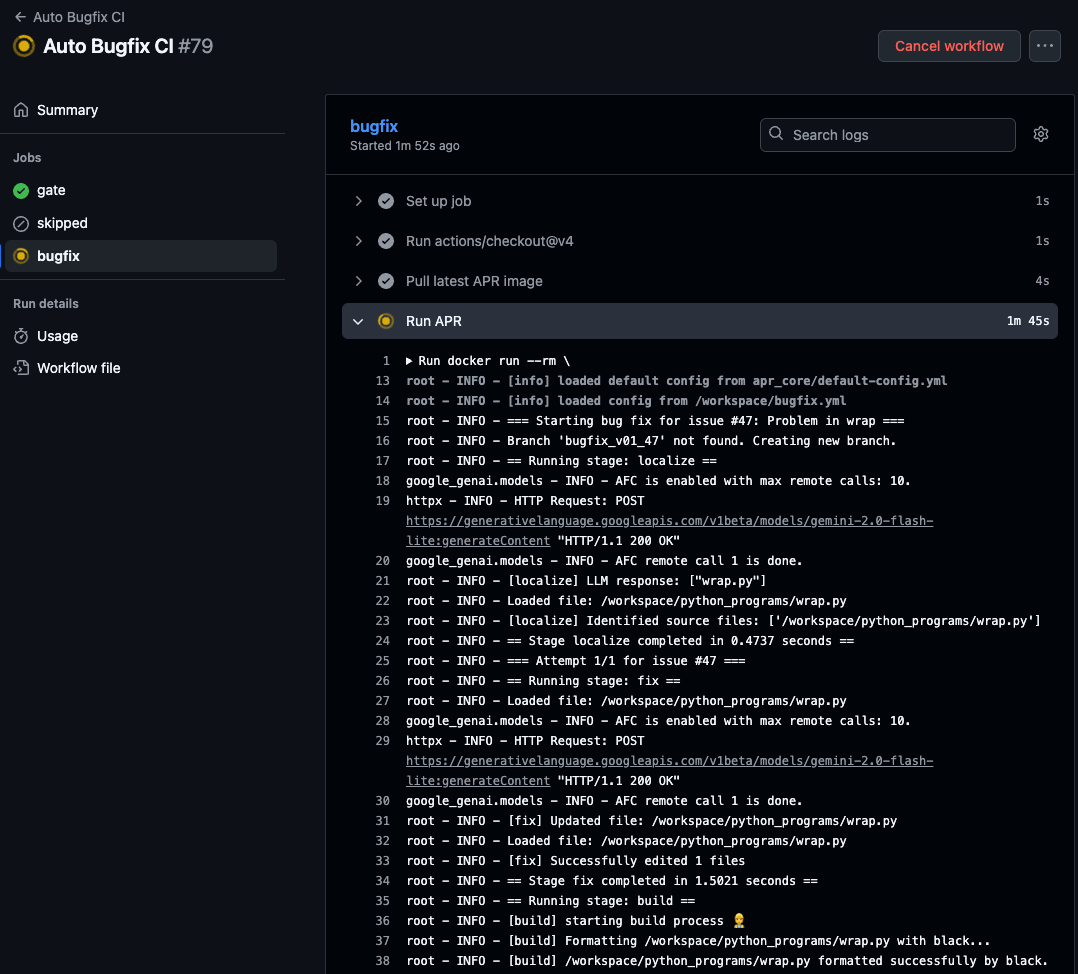
\includegraphics[width=1\textwidth]{images/workflow/logs.png}
    \caption{APR log stream}
    \label{fig:log-stream}
\end{figure}


\section{Evaluation Results}
The evaluation is based on the data collected during the execution of the prototype. This information is stored in the artifacts of the Github Actions run. Using the \textbf{get\_run\_data.py} script we collected the APR artifacts and the GitHub Pipeline information using the GitHub API. The script then processes the data and generates a report with the results of the evaluation. With the fetched data we calculate the metrics defined in %\ref{Evaluation}.

We evaluate X pipeline runs with X different LLMs. 

\begin{table}[ht]
    \centering
    \small
    \begin{tabular*}{\textwidth}{@{\extracolsep{\fill}} p{3.5cm} | p{2cm} | p{2cm} | p{2cm} | p{2cm} @{}}
        \toprule
        \textbf{Model} & \textbf{Repair Success Rate} & \textbf{Average Cost} & \textbf{Average Number of Attempts} & \textbf{Average Execution Time} \\
        \midrule
        \textbf{gemini-2.0-flash} & 92.5\% & 0.00 & 0.00 & 0.00s \\
        \textbf{gemini-2.5-flash-lite} & 95\% & 0.00 & 0.00 & 0.00s \\
        \textbf{gemini-2.5-flash} & 0.00\% & 0.00 & 0.00 & 0.00s \\
        \textbf{gemini-2.5-pro} & 100\% & 0.00 & 0.00 & 0.00s \\
        \textbf{gpt-4o} & 0.00\% & 0.00 & 0.00 & 0.00s \\
        \textbf{gpt-4.1-mini} & 0.00\% & 0.00 & 0.00 & 0.00s \\
        \textbf{claude-3-7-sonnet} & 0.00\% & 0.00 & 0.00 & 0.00s \\
        \textbf{claude-3-haiku} & 0.00\% & 0.00 & 0.00 & 0.00s \\
        \textbf{claude-sonnet-4-0} & 0.00\% & 0.00 & 0.00 & 0.00s \\
        \bottomrule
    \end{tabular*}
    \caption{Results of evaluation}
\end{table}

full artifacts are available in the repository in the Appendix \ref{Appendix}.

